Radioactivity is the process by which an unstable atomic nucleus decays through the emission of particles. This process is present in the Universe since the Big Bang. The formation of the Earth from the remains of supernova explosions explains why the different layers that make up the Earth contain radioactive elements. 

Humanity has always been exposed to ionizing radiation, both from the Earth's crust radioactivity and cosmic rays (external natural irradiation). The human body also contains radioactive elements such as $\ce{^{3}H}$, $\ce{^{14}C}$ and $\ce{^{40}K}$, introduced into it through food, water ingestion and air inhalation (internal natural irradiation). As it can be seen in Figure \ref{fig:RadioactiveDosePopulation}, most of the radioactive dose received by the population is due to both internal and external natural radioactivity, whose effective dose\footnote{The effective dose is the radioactive dose absorbed by the population, weighted by the radiosensitivity of each organ or tissue.} is estimated to be $2.42~\milli\sievert/$yr as shown in Table \ref{tab:RadioactiveNaturalDosePopulation}. 

\begin{figure}[h]
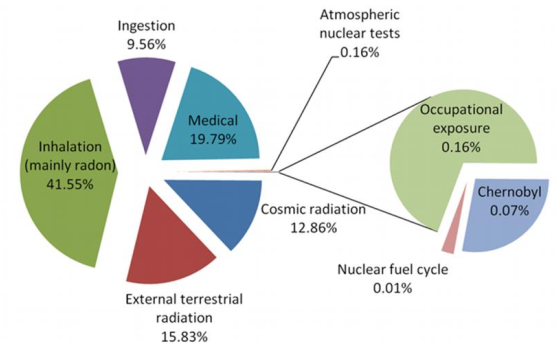
\includegraphics[scale=0.5]{2Introduction/RadioactiveDosePopulation.png}
\centering
\caption{Annual average distribution of the radioactive dose received by the population~\cite{IAEA}\label{fig:RadioactiveDosePopulation}.}
\end{figure}

\begin{table}[h]
\centering{}%
\begin{tabular}{lcc}
\toprule 
Radiation source & Eff. dose ($\milli\sievert/$yr) & Typical range ($\milli\sievert/$yr)\tabularnewline
\midrule
\midrule 
Cosmic (external) & $0.39$ & $0.3 - 1.0$ \tabularnewline
Terrestrial (external) & $0.48$ & $0.3-0.6$ \tabularnewline  
Inhalation (internal) & $1.26$ & $0.2-10$ \tabularnewline
Ingestion(internal) & $0.29$ & $0.2-0.8$ \tabularnewline
\midrule
Total & $2.42$ & $1-12.4$ \tabularnewline
\bottomrule
\end{tabular}
\caption{Annual average distribution of the effective dose received by the population due to natural radioactivity~\cite{UNSCEAR, CSN}.}
\label{tab:RadioactiveNaturalDosePopulation}
\end{table}

Since the discovery of radioactivity by Henri Becquerel in $1896$, lots of nuclear-based technologies were developed and applied to various fields such as Energy, Chemistry, Biology, Technology, Medicine, Industry, etc. Due to nuclear applications, a number of anthropogenic radioactive sources have emerged in society, resulting in radioactive elements released into the environment. It can be noticed in Figure \ref{fig:RadioactiveDosePopulation} that the most important part of the dose received by the population from artificial sources comes from medical practice. The growth of knowledge and the development of measurement techniques for radioactivity have provided evidence of the harmful effects of radioactivity on living organisms. This leads to the necessity of controlling the radiation to which the population is exposed, keeping it under safe limits. To accomplish this purpose, several organizations were created to propose recommendations for radiological protection to the different state organisms and governments at the international level. The main ones are:

\begin{enumerate}
\item{} The International Commission of Radiological Units and Measurements (ICRU) \cite{ICRU}, created during the first International Conference of Radiology held in London in 1925 to define concepts and units necessary to quantify the negative effects of radioactivity.

\item{} The International Commission on Radiological Protection (ICRP) \cite{ICRP}, created in 1928 by the International Society of Radiology (ISR) \cite{ISR}. The ICRP aims to make recommendations and provide guidance on different aspects of protection against radioactivity. The ICRP does not have the legal capacity to enforce its recommendations, but these are widely included in the legislation of most countries. %is fairly consistent with them.

\item{} The United Nations Scientific Committee on the Effects of Atomic Radiation (UNSCEAR) \cite{UNSCEAR}, created in 1955 with the goal of estimating and reporting the levels and effects of ionizing radiation on the population and the environment. These estimates are taken into account by governments worldwide to establish their safety standards.

\item{} The International Atomic Energy Agency (IAEA) \cite{IAEA}, created in 1957 to promote the peaceful use of nuclear energy and to avoid its use for military purposes such as nuclear weapons. Although established independently from the United Nations through its international treaty, the IAEA reports regularly to both the United Nations and the Security Council.

\item{} The European Atomic Energy Community (EURATOM), created in 1957, which is an international organization ruled by the EURATOM treaty. Its objective is to coordinate research programs for the peaceful use of nuclear energy and the sharing of knowledge, infrastructures and funding of nuclear energy.

\item{} The Nuclear Safety Council (CSN) \cite{CSN} of Spain, created in 1980, is the authority in Spain for nuclear safety and radiation protection. It has the objective of protecting employees, the general population and the environment from the harmful effects of ionizing radiation from anthropogenic origin. For this goal, the CSN ensures that nuclear and radioactive facilities are operated safely and establishes the preventive and corrective measures to be applied in radiological emergencies. The CSN manages two detector networks to control the levels of radioactivity in the environment and to assess the impact of radioactive facilities:

\begin{enumerate}
\item{} The network of automatic stations REA (Red de Estaciones Automáticas) \cite{REA}. The REA consists of several gamma detectors, distributed across the country as indicated in Figure \ref{subfig:REA}, which measure the radioactive dose in real time. The REA is employed for real-time detection of radiological issues to enable taking prompt safety measures.

\item{} The network of sampling stations REM (Red de Estaciones de Muestreo) \cite{REM}. The REM consists of a collection of points, shown in Figure \ref{subfig:REM}, from which samples are taken and measured in a laboratory. About twenty Spanish laboratories integrate this network. The objective of the REM is to characterize the concentration and evolution of radioisotopes present in the radioactive background of Spain and to quantify the impact of radioactive facilities on the environment.
\end{enumerate}

\begin{figure}
\centering
    \begin{subfigure}[b]{0.7\textwidth}
    \centering
    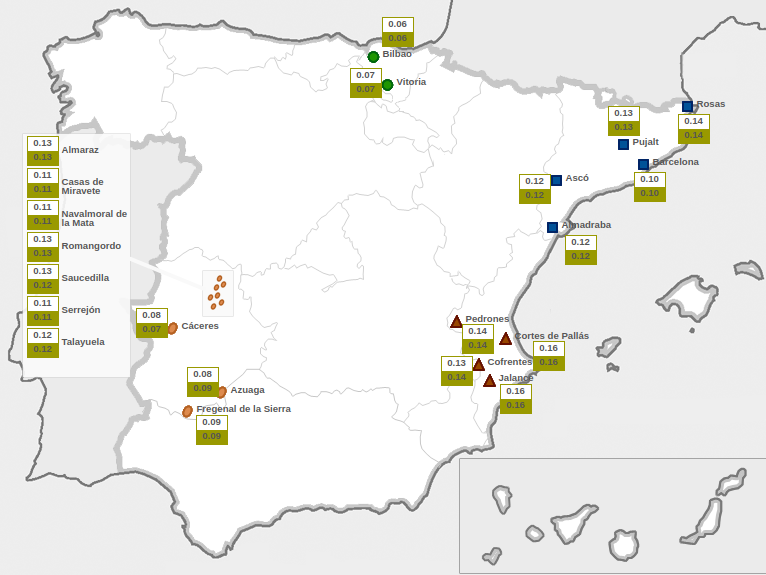
\includegraphics[width=\textwidth]{2Introduction/REA.png}  
        \caption{}\label{subfig:REA}
    \end{subfigure}
    \hfill
    \begin{subfigure}[b]{0.7\textwidth}
    \centering
    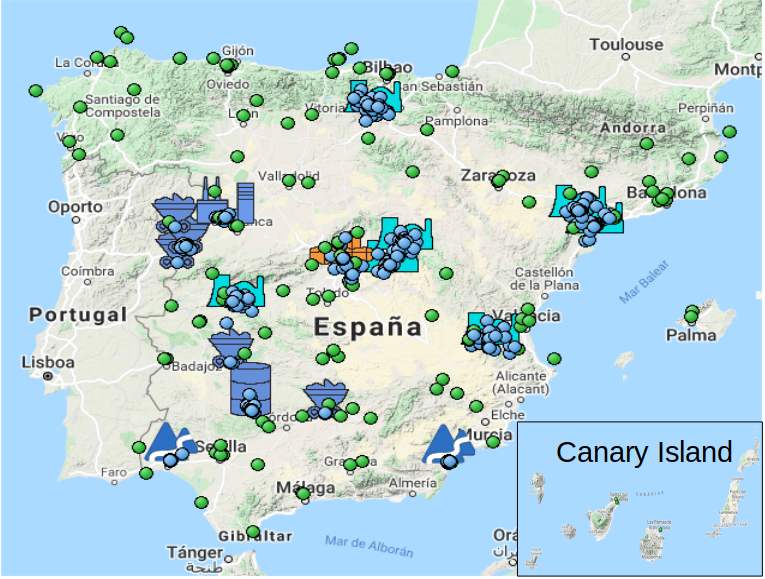
\includegraphics[width=\textwidth]{2Introduction/REM.png}  
    \caption{\label{subfig:REM}}
    \end{subfigure}
 \caption{Networks of automatic and sampling stations managed by the Spanish CSN. a) Measurement locations of the REA \cite{REA}. The white and green insets are the daily and monthly average of the gamma dose, respectively. b) Measurement locations of the REM \cite{REM}. Blue dots are locations near nuclear facilities, and green dots are locations uniformly distributed throughout the country.}
 \label{fig:NetworksCSN}
\end{figure}
%There are other networks that measure different parameters such as the concentration of $\ce{^{222}Ra}$ in the air. The measurements of all the networks complies with to the EUROTAM treaty \cite{100BqL}.

\end{enumerate}

The goal of the TRITIUM project is to develop a monitor capable of automatically measuring low levels of tritium in water in quasi-real-time\footnote{Quasi-real-time is an approximation of real-time measurements. It means a relatively small time, like less than $1~\hour$.}. This monitor is intended to be included in the REA.

Tritium is one of the radioactive isotopes routinely measured in REM tests. It is detected through the low-energy electrons produced in its beta decay, mainly using the Liquid Scintillation Counter technique (LSC). Due to the limitations of the current tritium detection techniques, described in section \ref{sec:StateOfTheArt}, the TRITIUM project was recently proposed with the objective of building a tritium detector based on scintillating fibres in contact with the water sample. The photons produced in these scintillating fibres are read out by photosensors, either photomultiplier tubes (PMTs) or silicon photomultipliers (SiPMs). The final emplacement of the TRITIUM monitor is a site close to the Arrocampo dam (Extremadura, Spain), whose water is used for the cooling system of the Almaraz nuclear power plant (NPP), located 4 km upstream from the Arrocampo dam. The monitor will be used to ensure that the tritium levels of the Arrocampo dam  water are below the legal limit of $100~\becquerel/\liter$ specified in the EURATOM Directive 2013/59/Euratom \cite{100BqL}. In addition, this will confirm the correct operation of the Almaraz NPP, since an increase of tritium activity released could indicate a malfunctioning of the reactor. This monitor could also be used in many different places with radioactive facilities like the future fusion power plants\footnote{The International Thermonuclear Experimental Reactor, ITER, will need up to several tens of kilograms of tritium to function, which corresponds to several $\tera\becquerel$ of activity.}, nuclear research facilities\footnote{Tritium is one of the main emissions from nuclear research facilities \cite{FERMILAB, BrookHavenNationalLaboratory}.} or tracking the pathway of tritium discharges to groundwater \cite{TrackingTritium}. 

Tritium is one of the most abundantly produced radioisotopes in an NPP, as it was verified in the United States Department of Energy (DOE) \cite{FiberDetector1a, FiberDetector1b}, in several research facilities in China \cite{CommonEmissionTritium} and places close to them (ground, surface and wastewater). Tritium is produced in the nuclear reactor cooling water system of NPPs by neutron capture of deuterium existing in the heavy water ($\ce{D_2 O}$), semi-heavy water ($\ce{H D O}$) or deuterium created by neutron capture in light water ($\ce{H_2 O}$). Tritium is finally released partially or totally into the environment in a quantity that depends on the reactor type, as shown in Table \ref{tab:TritiumEmisionsNPPs}. The most common form in which tritium is released into the environment is $\ce{HTO}$ \cite{CommonEmissionTritium}.
%All these processes have a large probability of happening due to the huge neutron flux, of the order of $10^{14} ~\ce{n} \, \cm^{-2} \second^{-1}$ in the nuclear reactor \cite{CrossSeccionNeutrons}

\begin{table}[htbp]
\centering{}%
\begin{tabular}{lcc}
\toprule 
Reactor type & Gaseous discharge ($\giga\becquerel/$y) & Liquid discharge ($\giga\becquerel/$y)\tabularnewline
\midrule
\midrule 
PWR & $3.70\cdot 10^{3}$ & $2.59\cdot 10^{4}$ \tabularnewline
BWR & $1.85\cdot 10^{3}$ & $3.70\cdot 10^{3}$ \tabularnewline
HWR & $7.40\cdot 10^{5}$ & $1.85\cdot 10^{5}$ \tabularnewline
GCR & $7.40\cdot 10^{3}$ & $1.11\cdot 10^{4}$ \tabularnewline
\bottomrule
\end{tabular}
\caption{Emission of tritium per year from different types of nuclear reactors: Pressurized Water Reactor (PWR), Boiling Water Reactor (BWR), Heavy Water Reactor (HWR) and Gas-Cooled Reactor (GCR) \cite{CommonEmissionTritium}.}
\label{tab:TritiumEmisionsNPPs}
\end{table}

NPPs are operational for more than 60 years and, nowadays, they are essential for providing a large part of the electric power used all over the world (more than $20\%$ in Spain \cite{PercentageEnergySpain} and more than $10\%$ in the world \cite{PercentageEnergyWorld}). Although the Spanish government is planning to progressively shut all NPPs down, there are other countries like China \cite{60ReactorsChina} or the United States \cite{35MillionsUSA} that promote their use. NPPs are a profitable investment since they are one of the cheapest sources of energy production. Their energy production rate is stable since it does not depend on meteorological conditions. Moreover, NPPs do not emit greenhouse gases. Although there are alternative energy sources which are being developed quickly (photovoltaic, wind, tidal energy, etc.), as well as other concepts of energy production and saving (local production, energy efficiency, smart cities, etc.), they are currently not enough to cover the population needs. However, NPPs have some important drawbacks such as contamination of fresh water from uranium mining, nuclear waste, nuclear proliferation and the risk of radioactive contamination from accidents as happened in the past: Chernobyl, Fukushima and Three Mile Island \cite{ThreeMileIsland}. In any case, world nuclear energy production is most likely not going to be stopped in the next decade. In fact, the United States Energy Information Administration (EIA) expects a future increase of nuclear energy production \cite{EIAOutlook}. Therefore, safety is not a negotiable aspect and there must be a development of safeguards, like alarm systems, that warn of any malfunction of NPPs. 

%which is normally done by liquid scintillation counter technic (LSC). This technic has a very good detection capability and precision but it has the inconvenient of providing a delayed results of about 1-2 days or even more. Liquid scintillation technique for the tritium measurement will be presented in section \ref{sec:StateOfTheArt}.